%-*- tex; tabsize:2; -*- %%%%%%%%%%%%%%%%%%%%%%%%%%%%%%%%%%%%%%%%%%%%%%%%%%%
%
%                          Copyright 2004-2005 JASSPA.
%                           All Rights Reserved
%
%
%  System        : MicroEmacs
%  Module        : user Manual
%  Object Name   : $RCSfile: jasspame.tex,v $
%  Revision      : $Revision: 1.3 $
%  Date          : $Date: 2005-03-11 21:12:42 $
%  Author        : $Author: jon $
%  Created By    : Jon Green
%  Created       : Mon Oct 25 21:36:13 2004
%  Last Modified : <050311.2110>
%
%  Description
%
%  Notes
%
%  History
%
%  $Log: not supported by cvs2svn $
%  Revision 1.2  2005/03/11 01:35:24  jon
%  Added User Setup information.
%
%  Revision 1.1  2005/03/10 01:00:55  jon
%  First draft of quick start document.
%
%
%%%%%%%%%%%%%%%%%%%%%%%%%%%%%%%%%%%%%%%%%%%%%%%%%%%%%%%%%%%%%%%%%%%%%%%%%%%%%
%
% Copyright (c) 2004-2005 JASSPA.
%
% All Rights Reserved.
%
% This  document  may  not, in  whole  or in  part, be  copied,  photocopied,
% reproduced,  translated,  or  reduced to any  electronic  medium or machine
% readable form without prior written consent from JASSPA.
%
%%%%%%%%%%%%%%%%%%%%%%%%%%%%%%%%%%%%%%%%%%%%%%%%%%%%%%%%%%%%%%%%%%%%%%%%%%%%%

\documentclass[11pt,a4paper,pdftex]{article}
% Bring in the CVS information.
\def\CVS$#1: #2 ${\expandafter\def\csname CVS#1\endcsname{#2}}
\CVS$Revision: 1.3 $ % or any CVS keyword
\CVS$Date: 2005-03-11 21:12:42 $

\usepackage{ifthen}                     % Conditional processing.

\newboolean{Colorlinks}
\setboolean{Colorlinks}{true}              % For colored links

% Document information
%\newcommand{\docAuthor}{Jon Green, Kevin Garvey}
\newcommand{\docAuthor}{Jon Green}
\newcommand{\docSubject}{JASSPA MicroEmacs}
\newcommand{\docTitle}{Getting Started with JASSPA MicroEmacs}
\newcommand{\docDate}{\CVSDate}
\newcommand{\docVersion}{\CVSRevision}
\newcommand{\docReference}{jasspame}

% Import the font packages.
%\usepackage[latin1]{inputenc}  % We do not seem to need this
\usepackage{eurosym}            % Use the Euro symbol for "\euro"
\usepackage[T1]{fontenc}        % Refer to TeX psnfss2e.pdf
\usepackage{textcomp}           % Refer to TeX psnfss2e.pdf
\usepackage{aecompl}            % AE complement to T1 for "\NG" and "\ng"
\usepackage{color}
%
% FONTS: The document is typeset in the following fonts:-
% roman:      Times-Roman
% sans serif: Helvetica (scaled at .92)
% typewriter: Courier
\usepackage{courier}
\usepackage[scaled=0.92]{helvet}
%\usepackage{utopia}
\renewcommand{\rmdefault}{ptm}  % Roman font is Times-Roman
%\renewcommand{\rmdefault}{put}  % Utopia font is Times-Roman
\renewcommand{\sfdefault}{phv}  % Sans serif font is helvetica
\renewcommand{\ttdefault}{pcr}  % Typewriter font is courier

% Change the default font to Helvetica.
%\usepackage{bookman}
%\renewcommand{\familydefault}{\sfdefault}
%\renewcommand{\sfdefault}{ppl}

% Import the font packages.
\usepackage{pslatex}
\usepackage{longtable}                  % Long split table environment.
\usepackage{graphicx}                   % Picture import package
\usepackage{fancyhdr}                   % Use fancy headers
\usepackage[numbers]{natbib}            % Use Natural Sciences Citations and References

% Detect, if we are using pdftex to create pdf output. The following
% code should better be in a LaTeX package...
\makeatletter
\newif\ifpdfoutput
\@ifundefined{pdfoutput}%
  {\let\pdfoutput\@undefined}%
  {\ifcase\pdfoutput
     \let\pdfoutput\@undefined
   \else
     \pdfoutputtrue
   \fi
  }%
\makeatother

\usepackage{geometry,mflogo,xspace,path,bm}
\newcommand{\psext}{ps}
\newcommand{\pdfext}{pdf}
\newcommand{\dviext}{dvi}

% Set up the default link colour
\ifthenelse{\boolean{Colorlinks}}
{%
  \newcommand{\Linkcolor}{blue}
  \newcommand{\Citecolor}{red}
  \newcommand{\Urlcolor}{blue}
}
{%
  \newcommand{\Linkcolor}{black}
  \newcommand{\Citecolor}{black}
  \newcommand{\Urlcolor}{black}
}

\ifpdfoutput
  \pdfcompresslevel9
  \usepackage[colorlinks,bookmarks]{hyperref}
  \hypersetup{
    pdfauthor={\docAuthor},
    pdftitle={\docTitle},
    pdfsubject={\docSubject},
    pdfcreator={SunOS 5.9(sparc) - e-TeX(Web2C 7.5.2)},
    pdfkeywords={Emacs,MicroEmacs,Me,JASSPA},
    linkcolor={\Linkcolor},
    citecolor={\Citecolor},
    urlcolor={\Urlcolor},
    bookmarksnumbered=true,
    bookmarksopen=true
  }
  \usepackage{thumbpdf}
  \let\docext=\pdfext
\else
  \let\docext=\dviext
  \usepackage[bookmarks]{hyperref}
\fi

\title{\docTitle}
\author{Jon Green}
\date{\docDate}
%
% Bottom of the pages are ragged.
\raggedbottom
%
% Change the page width
%
\setlength{\marginparsep}{0pt}
\setlength{\marginparwidth}{0pt}
\addtolength{\textwidth}{.75in}
\addtolength{\hoffset}{-.25in}

\pagestyle{fancy}
% Set up the page.
% There is 1 inch at the top, reduce this to 0.4 inch.
\addtolength{\voffset}{-.6in}
\addtolength{\textheight}{.6in}
% We are adding a 1/2 inch graphic adjust the page sizes.
\setlength{\headheight}{.5in}
% Push page length to the bottom.
\addtolength{\textheight}{.5in}

%% Save the header image in a box
\newsavebox\HeaderImage
\savebox\HeaderImage{
\includegraphics[keepaspectratio,height=0.5in]{logo}}
% Redefine the header and footer for an alternative style.
\renewcommand{\sectionmark}[1]{\markright{\thesection\ #1}}
\fancyhf{}          % Delete the current header and footer
\fancyhead[EL,OR]{\bfseries\docTitle \\ \bfseries\rightmark}
\fancyhead[LO,RE]{\usebox{\HeaderImage}}
\fancyfoot[OL,ER]{{\small{Copyright {\textcopyright} 2004-2005 JASSPA.}}\linebreak
                   \textit{\small{\docReference~~v\docVersion~~\docDate}}}
\fancyfoot[EL,OR]{\textsf{\large \textbf{\thepage}}}
\renewcommand{\headrulewidth}{1.5pt}%
\renewcommand{\footrulewidth}{1.5pt}%

% Redefine a plain header and footer than is absent for the
% front page.
\fancypagestyle{plain}{%
  % Watermark for the first header. First we clear down the
  % existing header that may be defined.
  \fancyhead{}%
  % Refer to the "Using Imported Graphics in LaTeX2"
  % Define the header to appear on the left hand edge of the page.
  % The picture dimensions are specified as (0,0), this means that
  % it occupies zero space (as far as the layout engine is concerned).
  % Appearing in the header means that they are rendered before the
  % page itself.
  % The image is placed 0 inches to the left and -10inches below
  % the header. The graphics are then included such that the
  % aspect ratio is maintained and the image width is as wide as
  % the text width.
  \fancyhead[OL,ER]{\setlength{\unitlength}{1in}
%             \begin{picture}(0,0)
%               \put(0,-10){\includegraphics[keepaspectratio,width=\textwidth]{watermark}}
%             \end{picture}
  }
  \renewcommand{\headrulewidth}{0pt}  % Remove line
  \fancyfoot[EL,OR]{}
}

\newcommand{\tableTitle}[1]{\textbf{#1}}%   % used on all table titles.

\begin{document}
\pagenumbering{roman}           %%% Roman page numbers for ToC

%%%%%%%%%%%%%%%%%%%%%%%%%%%%%%%%%%%%%%%%%%%%%%%%%%%%%%%%%%%%%%%%%%%%%%%%%%%%%%
% New commands
\definecolor{CodeColor}{rgb}{0.95,0.95,0.95}
\newcommand{\CodeInsert}[1]{%
\vspace{3pt}
\colorbox{CodeColor}{\parbox{\textwidth}{\texttt{#1}}}
\vspace{3pt}
}

%%%%%%%%%%%%%%%%%%%%%%%%%%%%%%%%%%%%%%%%%%%%%%%%%%%%%%%%%%%%%%%%%%%%%%%%%%%%%%
%  Title Page                                                                %
%%%%%%%%%%%%%%%%%%%%%%%%%%%%%%%%%%%%%%%%%%%%%%%%%%%%%%%%%%%%%%%%%%%%%%%%%%%%%%
\thispagestyle{plain}
% The top header is the document information and the company logo. This is
% made up of 2 parbox's to get the correct horizontal wrapping that is
% required.
\parbox{2in}{
\includegraphics[keepaspectratio,width=1.9in]{logo}}
\hfill
\parbox{3.25in}{\sloppy
                \hfill\textsf{\huge JASSPA}
                \begin{flushright}
                  \textsf{\textbf{\Huge \docTitle}}
                \end{flushright}
                \hfill\textsf{\huge Version \docVersion}

                \hfill\textsf{\docAuthor}}
% The text information at the bottom of the page containing a copyright notice
% and contact details. This placed in a table and then shunted to the bottom
% of the page.
\begin{table}[b]
  \begin{center}
    \begin{tabular}{p{3in}p{3in}}
      \textsf{JASSPA}\vspace{6pt} & \\
      \textsf{\href{http://www.jasspa.com}{www.jasspa.com}\newline
              \href{mailto:support@jasspa.com}{support@jasspa.com}} & \\
%      \textsf{\sloppy\textbf{Copyright Notification:} No part of this
%      publication may be reproduced except as authorised by written
%      permission. The copyright and the foregoing restriction extend to
%      reproduction in all media.}
    \end{tabular}
  \end{center}
\end{table}

%%%%%%%%%%%%%%%%%%%%%%%%%%%%%%%%%%%%%%%%%%%%%%%%%%%%%%%%%%%%%%%%%%%%%%%%%%%%%%
%  Revision History                                                          %
%%%%%%%%%%%%%%%%%%%%%%%%%%%%%%%%%%%%%%%%%%%%%%%%%%%%%%%%%%%%%%%%%%%%%%%%%%%%%%
\newpage
% Change the format of the document to European paragraph spacing.
\setlength{\parindent}{0pt}
%\setlength{\parskip}{1ex plus 0.5ex minus 0.2ex}
\setlength{\parskip}{0.5ex}
\pagestyle{fancy}

\begin{small}
\vspace{.5in}
JASSPA.
\href{http://www.jasspa.com}{www.jasspa.com}\newline
\href{mailto:support@jasspa.com}{support@jasspa.com}\newline

\vspace{0.5in}

\textit{Copyright \textcopyright\ 2004-2005 JASSPA.}

% \textit{Copyright}

\vspace{0.5in}

\begin{table}[ht]
  \begin{tabular}{ll}
    Title:        & \docTitle \\
    Reference:    & \docReference \\
    Version       & v\docVersion \\
    Date:         & \docDate \\
  \end{tabular}
\end{table}

Typeset with the TexLive 2004 \LaTeX\ Documentation System under Sun Solaris 9.

\vspace{0.5in}

\begin{center}
  \begin{table}[ht]
    \begin{tabular}{|c|c|p{4in}|c|}
    \hline
    \tableTitle{Date} & \tableTitle{Who} & \tableTitle{Description} & \tableTitle{Revision} \\
    \hline
    2004/10/25 & Jon & Draft. & 1.00 \\ \hline
    \end{tabular}
  \end{table}
\end{center}
\end{small}

%%%%%%%%%%%%%%%%%%%%%%%%%%%%%%%%%%%%%%%%%%%%%%%%%%%%%%%%%%%%%%%%%%%%%%%%%%%%%%
% Introduction                                                               %
%%%%%%%%%%%%%%%%%%%%%%%%%%%%%%%%%%%%%%%%%%%%%%%%%%%%%%%%%%%%%%%%%%%%%%%%%%%%%%
\newpage
% Change the format of the document to European paragraph spacing.
\setlength{\parindent}{0pt}
%\setlength{\parskip}{1ex plus 0.5ex minus 0.2ex}
\setlength{\parskip}{0.5ex}
\pagestyle{fancy}

%\textbf{\Large Preface}
\pdfbookmark[1]{Preface}{intro}    %%% additional bookmark for ref
\markboth{Preface}{Preface}   %%% for the page header
\section*{Preface}
%\addcontentsline{toc}{section}{\numberline{}Preface}

Time is short, armed with a reasonable \LaTeX\ boiler plate it is time to put
down some usable notes on getting up and running with JASSPA MicroEmacs. The
on-line help that comes with JASSPA MicroEmacs details every public function
and variable in the editor however it is not that accessible and certainly
does not help the new user.

In this first draft, that will undoubtedly grow over time, we simply present
the post installation configuration to help the new user get up and running
with the editor.

Jon Green\newline
25th October 2004.

%%%%%%%%%%%%%%%%%%%%%%%%%%%%%%%%%%%%%%%%%%%%%%%%%%%%%%%%%%%%%%%%%%%%%%%%%%%%%%
% Table of Contents                                                          %
%%%%%%%%%%%%%%%%%%%%%%%%%%%%%%%%%%%%%%%%%%%%%%%%%%%%%%%%%%%%%%%%%%%%%%%%%%%%%%

\newpage
\pdfbookmark[1]{Contents}{toc}          %%% additional bookmark for ToC
\markboth{Table of Contents}{Table of Contents} %%% for the page header
\tableofcontents
\newpage

%%%%%%%%%%%%%%%%%%%%%%%%%%%%%%%%%%%%%%%%%%%%%%%%%%%%%%%%%%%%%%%%%%%%%%%%%%%%%%
% References                                                                 %
%%%%%%%%%%%%%%%%%%%%%%%%%%%%%%%%%%%%%%%%%%%%%%%%%%%%%%%%%%%%%%%%%%%%%%%%%%%%%%

\cleardoublepage
% Page numbering - continue the page numering from the arabic space. When we
% change to arabic space then the counter value is reset. Create a temporary
% counter to hold the page value from the `Roman' page space so that we
% commence the page numbering in `Arabic' space from where we left it. This
% technique ensures that the PDF page numbering is identical to that specified
% in the document.
\newcounter{pagetemp}                   % Temporary counter.
\setcounter{pagetemp}{\value{page}}     % Snoop the Roman page numbers
\pagenumbering{arabic}                  % From now on Arabic page numbers
\setcounter{page}{\value{pagetemp}}     % Align with Roman

% Change the format of the document to European paragraph spacing.
\setlength{\parindent}{0pt}
%\setlength{\parskip}{1ex plus 0.5ex minus 0.2ex}
\setlength{\parskip}{0.5ex}

\section{Installation and Setup}

\subsection{Installation}

To install JASSPA MicroEmacs then download the appropriate bundle from
\href{http://www.jasspa.com}{www.jasspa.com}. Most of the common platforms
include packages to simplify installation.

\subsubsection{Packaged Sun Solaris}

  As root install the package.

\CodeInsert{%
cd /tmp\newline
unzip jasspa-mepkg-sun-sparc-59-\textit{yyyymmdd}.zip\newline
pkgadd -d jasspa-me}

  The package is installed in \texttt{/opt/jasspa}. Edit your local login
  script file to include the executable on your local path e.g.
  \texttt{.cshrc} or \texttt{.profile} -- the syntax depends on the shell type
  that you use.

\CodeInsert{%
\#\newline
\# Set up Microemacs\newline
\#\newline
if [ -d /opt/jasspa ] ; then\newline
\hspace*{2em}PATH=\$PATH:/opt/jasspa/bin\newline
\hspace*{2em}MANPATH=\$MANPATH:/opt/jasspa/man\newline
fi\newline
...\newline
export PATH}

  The package may be subsequently removed using:

\CodeInsert{pkgrm jasspa-me}

\subsubsection{Packaged Red Hat Linux/Fedore Core}

  As root install the package.

\CodeInsert{rpm -i jasspa-me-\textit{yyyymmdd}-1.i386.rpm}

  The package is installed in directory \texttt{/usr/share/jasspa}, the
  executable is installed in \texttt{/usr/bin} and requires no additional
  setup.

  The package may be subsequently removed using:

\CodeInsert{rpm -e jasspa-me}

\subsubsection{Packaged HP-UX}

  For HP-UX then the package may be installed via SAM, but is easier to
  install using the command line:

\CodeInsert{/usr/sbin/swinstall -s `pwd`/jasspa-mepkg-hpux-pa-10.20-\textit{yyyymmdd}.depot jasspa-me}

  The package is installed in \texttt{/opt/jasspa}. The executable is
  automatically added to the shell profile environment. The user should log
  out and log back in again to pick up the new environment settings which are
  added to \texttt{/etc/profile}.

  The package may be subsequently removed using:

\CodeInsert{swremove jasspa-me}

\subsubsection{Packaged Microsoft Windows}

  Microsoft Windows environments 95/98/NT/2K/XP use an \textit{Install Shield}
  package installation which may be used to add and remove the package. The
  software is installed into \texttt{c:$\backslash$Program
  Files\-$\backslash$JASSPA\-$\backslash$MicroEmacs}.

  Unpack the \textit{zip} file, run \textbf{setup.exe} and follow the
  installation procedure.

\subsubsection{Non-packaged UNIX/Linux/BSD - System wide}

  For other UNIX/BSD environments where no package is provided then a manual
  installation is performed. Select the installation directory i.e.
  \texttt{/usr/local}.

\CodeInsert{cd /usr/local\newline
gunzip -c /\textit{path-to}/jasspa-metree-\textit{yyyymmdd}.tar.gz | tar xvf -}

    or using GNU tar

\CodeInsert{cd /usr/local\newline
gtar zxvf /\textit{path-to}/jasspa-metree-\textit{yyyymmdd}.tar.gz}

  The directory \texttt{/usr/local/jasspa} should now exist. Unpack the binary
  into the new directory and make it executable.

\CodeInsert{cd /usr/local/bin\newline
gunzip -c /\textit{path-to}/jasspa-me-linux-2.\textit{x}-\textit{yyyymmdd}.gz > me\newline
chmod a rx me}

  The installation is complete and you may now execute your favorite editor
  me.

\subsubsection{Non-packaged UNIX/Linux/BSD - User Installation}

  For other UNIX/BSD environments where a local user install is required (i.e.
  the user has no permissions to write to the system directories) then the
  following steps may be followed.

  Unpack \textit{metree} in your home directory, this creates a directory tree
  called \textbf{jasspa}, once unpacked then rename the directory to
  \textbf{.jasspa}.

\CodeInsert{cd $\sim$\newline
gunzip -c /\textit{path-to}/jasspa-metree-\textit{yyyymmdd}.tar.gz | tar xvf -\newline
mv jasspa .jasspa}

  Add downloaded spelling dictionaries by unpacking them into the
  \texttt{$\sim$/.jasspa/spell} subdirectory. Install the binary into your local
  binary directory - we assume \texttt{$\sim$/bin} e.g.

\CodeInsert{cd $\sim$/bin\newline
gunzip -c /\textit{path-to}/jasspa-me-linux-2.\textit{x}-\textit{yyyymmdd}.gz > me\newline
chmod a+rx me}

  Assuming that the binary directory is already on the users path then the
  installation is complete.

\subsubsection{MS-DOS}

  For MS-DOS then no installation script is provided and a manual installation
  is performed. Select the installation directory, we shall assume
  \texttt{c:$\backslash$jasspa}.

  Unpack the \texttt{metree} zip package to form the macro tree, this creates
  the directory \textit{jasspa}.

\CodeInsert{c:\newline
cd $\backslash$\newline
unzip jasspa-metree-\textit{yyyymmdd}.zip}

  The binary is placed in the \texttt{c:$\backslash$jasspa} directory. It is
  important that the binary is placed in the JASSPA tree as this allows the
  executable to locate the \textit{macros} and \textit{spelling} directories
  without any further configuration. If the binary is placed in a separate
  location from the tree then the \textit{\$MExxxPATH} environment variables
  must be defined to enable the editor to locate the tree.

  Two different binaries are provided which are built with DJGPP V1.0 and
  V2.0. If you have DJGPP V2.0 installed in your system then install the V2.0
  binary, otherwise install the V1.0 binary (as this is a self contained
  executable and has no run-time library dependencies).

\CodeInsert{cd $\backslash$jasspa\newline
unzip jasspa-me-msdos-djgpp1-\textit{yyyymmdd}.zip}

  The location of the executable should be added to the \texttt{autoexec.bat}
  file e.g.

\CodeInsert{SET PATH=\%PATH\%;c:$\backslash$jasspa}

  The system may be re-booted and the editor should be available on the
  command line \texttt{me}.

\subsubsection{Windows Manual Installation}

  Manual installation is required under \textbf{Win32s} and may be optionally
  performed in \textbf{Win32} environments (95/98/NT/2K/XP). This is very
  similar to the \textbf{MS-DOS} installation.

  Unpack the \texttt{metree} zip package to form the macro tree, this creates
  the directory \textit{jasspa}. This is typically extracted to
  \textit{c:$\backslash$Program Files} (\textbf{Win32s} may use
  \textit{c:$\backslash$me}).

\CodeInsert{c:\newline
cd "$\backslash$Program Files"\newline
unzip jasspa-metree-\textit{yyyymmdd}.zip}

  The executable is placed in the \textit{jasspa} directory:

\CodeInsert{cd "$\backslash$Program Files$\backslash$jasspa"\newline
unzip jasspa-me-win32-\textit{yyyymmdd}.zip
}

  Unlike \textbf{MS-DOS} then short cuts are typically used to launch the
  editor. The editor short-cut is typically edited with command line option
  \textbf{-c} to restore the previous session when launched.

\subsubsection{Spelling Dictionaries}

  The spelling dictionaries are downloaded separately and are not included in
  the base packages, multiple dictionaries may be downloaded and installed for
  each language to be supported. Some languages include a \textit{base} and
  \textit{extended} dictionary, the \textit{base} contains the most popular
  words, the \textit{extended} includes more obscure words over and above the
  \textit{base}. The \textit{base} and \textit{extended} dictionary are
  packaged together, but the \textit{extended} dictionary may be removed when
  downloaded to conserve disk space.

  The spelling archive contains both the dictonaries and language specific
  macros required to install the dictionary into the system. All of the
  dictionaries are derrived from \textit{ispell} dictionaries. The Copyrights
  for each of the dictionaries are contained in the macro files.

  To install then the archive is unpacked into the \textit{jasspa/spelling}
  directory that was created when \textit{metree} was unpacked. Simply unpack
  the contents of the archive into this directory.

\CodeInsert{cd /\textit{path-to}/jasspa/spelling\newline
unzip enus.zip}

  With the directory installed then set up MicroEmacs using \textbf{Help
  $\rightarrow$ User Setup} or from the command line \textbf{M-x user-setup}.

  \begin{itemize}
    \item Select the \textbf{Platform} tab.

    \item Select the \textbf{Language} from the drop-down box.

    \item Enable \textbf{Auto Save Dictionaries} to automatically save the
    dictionary when new words are added or ignored.

    \item Enable \textbf{Enable Auto-Spell} if the auto spell facility is
    required. Auto-Spell performs background spell checking and highlights
    erroneous words.

  \end{itemize}

\subsection{Building from Source}

  Where a particular platform does not exist then MicroEmacs may be built from
  source. It is expected that the environment is set up with the appropriate
  tools to perform the build.

  A simple build script is provided for both UNIX and DOS/Windows systems
  called \textbf{build}. Download the source bundle
  \texttt{jasspa-mesrc-\textit{yyyymmdd}} and unpack, this will create a
  directory \textbf{meYYMMDD}. Change directory to \textbf{src} and issue a
  build command:

\CodeInsert{\# DOS\newline
c:> build}

\CodeInsert{\# UNIX\newline
>sh> ./build}

  On most systems then the \textbf{build} will be performed, alternatively
  explicit make may be performed. A selection of make files exist for the
  different platforms \textbf{.mak} indicates the native platform compiler and
  \textbf{.gmk} indicates a GNU compiler.

\CodeInsert{make -f \textit{platform}.mak}

  The platform specific makefiles may be modified with compiler specific
  options for the target platform to produce a optimal executable.

  For Microsoft Windows environments then a Microsoft Project file is
  provided.

\subsection{Running For the First Time}

  On running MicroEmacs for the first time with the command \textbf{me} then
  the user is asked to set up the environment. This process collects some very
  basic information and creates the user private files that store context and
  state. The user may decline to perform the set-up and is prompted next time
  the editor is executed.

  The environment is analyzed and the system directory locations and search
  paths are determined. These can typically be accepted as is.

  \begin{itemize}

    \item \textbf{Enter you full name ?} This is \textit{your} name that is
    inserted in the header files that identify you as the author.

    \item \textbf{Set up the company file (y/n) ?} If you are working in a
    company environment then this allows you to enter the name of the company
    that is used in copyright statements automatically inserted into new
    headers etc.

    \item \textbf{Name the company file ?} This is the name of the macro file
    that stores company wide company information. The default is simply called
    \textbf{company} and is typically accepted. If you are using a site wide
    installation then your system administrator may set up a specifically
    named file which should be entered here.

    \item \textbf{Company Name ?} is the long name of the company i.e.
    \textit{Acme Building Inc.}

  \end{itemize}

  The configuration is complete and the top level help page is displayed. The
  user should now perform the \textbf{User Setup} step detailed in a later
  section.

\subsection{Help Information}

  The help information is available on-line and may be accessed using the
  mouse or the keyboard.

\subsubsection{Mouse Interaction}

  \textbf{Help$\rightarrow$General Help}

  The links are shown highlighted and may be traversed with the mouse by
  selecting the link with a double click.

\subsubsection{Keyboard Interaction}

  \textbf{esc-x help}

  The links may be traversed using the TAB key to move to the next link, a
  RETURN on the link causes the link to be followed.

\subsection{User Setup}

  On completion of the basic configuration then a certain amount of
  customization is typically required. The \textit{User Setup} dialog allows
  the user to perform this process and is invoked as follows:

  \textbf{esc-x user-setup} $\dots$ \textit{OR}\newline
  \textbf{Help$\rightarrow$User Setup}

\begin{figure}[!hbt]
  \begin{center}
    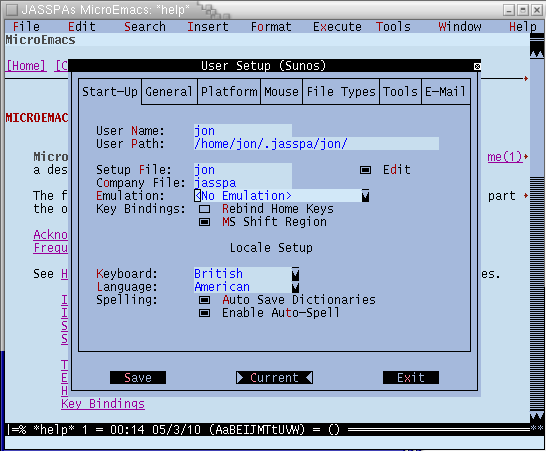
\includegraphics[keepaspectratio,height=3in]{usersetup}
    \caption{User Setup Dialog}
    \label{fig:usersetup}
  \end{center}
\end{figure}

  Navigation within the dialog is performed using the mouse and/or
  \texttt{TAB} and cursor keys. The \texttt{SPACE} key is used to open a drop
  down dialog. The configuration may be saved permanently using \textbf{Save}
  and installed into the current session using \textbf{Current}.

\subsubsection{Common Options}

  For a quick setup then the \textit{User Setup} dialog is traversed by pane,
  the most common options are described below, other options may be ignored.

  \begin{itemize}
    \item \textbf{Start-up} -- start up configuration information.

    \begin{itemize}

      \item \textbf{Emulation} select the preferred emulation mode of the
      editor. The standard key bindings are adjusted to be more consistent
      with the selected emulation.

      \item \textbf{Re-bind Home Keys} when disabled then the keys
      \textit{Home} and \textit{End} move to the beginning and end of the
      buffer respectively. When enabled then \textit{Home} and \textit{End}
      move to the beginning and end of the line respectively.

      \item \textbf{MS Shift Bindings} enabled performs Microsoft region
      selection using the cursor keys whilst the \texttt{SHIFT} key is
      pressed.

      \item \textbf{Keyboard} select your keyboard type, the keyboard bindings
      are corrected for the locale.

      \item \textbf{Language} the default spelling language. This has no
      effect if the dictionaries are not loaded.

      \item \textbf{Auto Save Dictionaries} typically enabled, causes the user
      defined spelling dictionary to be automatically saved on exiting the
      editor.

      \item \textbf{Enable Auto-spell} enable this option to allow MicroEmacs
      to perform spell checking whilst you type. Spelling errors are
      highlighted to indicate errors. With the mouse right click on the
      mis-spelt word and select an auto correction.

      \textbf{M-x auto-spell-buffer} to automatically spell check the
      whole buffer.

      \textbf{M-x spell-buffer} to spell check the buffer via spell dialog.

    \end{itemize}

    \item \textbf{General} -- general defaults and settings.

    \begin{itemize}

      \item \textbf{Full Name} user name that is inserted into new file
      templates

      \item \textbf{Main Menu} disable if the Main Menu is not required.

      \item \textbf{Alt Action} defines the behavior of the \texttt{ALT} key.
      Enable \textbf{Esc Prfx} if the \texttt{ALT} key may be used as a
      \texttt{ESC} key prefix (most Emacs users). Disable \textbf{Main menu
      Hot-keys} if the \texttt{ALT} key should not be used as a hot key to the
      Main menu. When both are enabled then the Main menu has priority.

      \item \textbf{Abbrev Setup} defines the behavior of the abbreviation key
      binding \textbf{esc esc}.

      \begin{itemize}

        \item Enabling \textbf{Accent} completes accented characters i.e.
        \texttt{:o<esc><esc>} is converted to a umlaut.

        \item Enabling \textbf{Lookback} attempts to complete the word based
        on previous words in the buffer. A further \textbf{esc esc} finds the
        previous etc.

        \item Enabling \textbf{Dict'n} attempts to complete a word based on
        the spelling dictionary.

      \end{itemize}

      \item \textbf{Tab to Indent} controls the behavior of the TAB key. By
      default, where indent rules exist for a buffer then the TAB key causes
      the indentation of the line to be re-evaluated rather than inserting a
      literal TAB character. Select the operation required, the default is
      \textit{Always Indent}.

    \end{itemize}

    \item \textbf{Platform} -- general platform specific settings.

    \begin{itemize}

      \item \textbf{Termcap Color (Termcap Only)} enables use of colors.

      \item \textbf{Use Fonts (Termcap Only)} enables use of \textbf{bold} and
      \underline{underline} fonts.

      \item \textbf{Font Name} selection of an alternative fixed font. For
      UNIX then use \textbf{xfontsel} to select a font to paste into the
      window. For MS-Windows then use the \textbf{Choose Font} button to
      select the font.

      \item \textbf{Enable Tool Bar} enable if the tool bar at the left of the
      screen is required. Add tools to the tool bar, this provides short cuts,
      itemized lists for specific buffers. The tool bar is buffer sensitive.

      \item \textbf{Ignore files} the list of files to be ignored in directory
      listings.

      \item \textbf{Fence Display} defines the behavior of the cursor at fence
      characters (i.e. \texttt{(,\{,\},),..}). \textbf{Always draw and jump on
      close} is the most popular, the brackets are colorized and the cursor
      jumps to the opening fence on entering a close. A miss-matched fence is
      highlighted in an error color.

      \item \textbf{Scroll Bars} generally \textbf{Wide with Splitter} is
      preferred in windowing environments.

      \item \textbf{Horizontal Scroll} defines the behavior of horizontal
      scrolling when the cursor is moved to the end of the line. By default
      only the current line is scrolled.

      \item \textbf{Vertical Scroll} defines the behavior of vertical
      scrolling when the cursor is moved down at the top/bottom line of the
      window. For terminals then \textbf{Default, half screen} is preferred,
      for windowing environments then \textbf{Smooth, Single line} is
      preferred.

      \item \textbf{Color Scheme} the highlighting color of the buffer window.
      In a console environment then use the special scheme for
      \textit{Termcap}.

    \end{itemize}

    \item \textbf{Mouse} -- behavior of the mouse.

    \begin{itemize}

      \item \textbf{Mouse Button Bindings} control the action on pressing a
      button, optionally in conjunction with the \texttt{SHIFT},
      \texttt{CONTROL} and \texttt{ALT} modifier keys. The wheel mouse setting
      is bound here.

    \end{itemize}

  \end{itemize}
  
\subsection{MicroEmacs Integration}

  This section discusses how MicroEmacs may be integrated with the desktop 
  environment and other tools.

\subsubsection{Desktop Integration}    

  Integration of MicroEmacs with the Window Manager desktop environment.

  \begin{itemize}

    \item Drag and Drop is supported. When a file(s) is dragged over a buffer
    window and released then the file(s) is opened in the drop window. 
    
    \textbf{UNIX} environments support \textit{Xdnd}. Under X-Windows the
    MicroEmacs window is not raised following the drop.
    
    \textbf{Microsoft Windows} the MicroEmacs window is raised following
    a drop operation.

    \item Different size bitmaps are provided for the desktop. 
    
    \textbf{UNIX} icons are provided in
    \texttt{\textit{/path-to}/jasspa/pixmaps} in both \textbf{png} and
    \textbf{pixmap} format. A set of additional file type MicroEmacs icons may
    be downloaded for use with Gnome, KDE and CDE.

    \textbf{Microsoft Windows}  different size bitmaps are provided in the icon executable file
    \textbf{meicons.exe}. This executable contains the standard JASSPA icon in
    addition to the file type icons. Select icons from this executable when 
    assigning MicroEmacs to specific file extensions. 

    \item When assigning MicroEmacs to a desktop icon then it is advisable to
    start MicroEmacs with the command line option \textbf{-c}. This option
    restores the editor to the previously loaded state of the last saved
    session.

    \item Where MicroEmacs is assigned as an open action for a given file type
    or extension then an existing editor session may be used rather than
    opening a new editor. To enable MicroEmacs reuse and existing session then
    invoke \textbf{me} with the \textbf{-o} command line option and enable the
    \textbf{Client-Server} configuration option (\textbf{Help $\rightarrow$
    User Setup $\rightarrow$ Platform $\rightarrow$ Client Server}). 
    
  \end{itemize}

\subsubsection{Tools Integration}
    
  MicroEmacs may be invoked from other tools as the selected text editor (i.e.
  \textbf{WinZip}). Multiple files may be specified on the command line for
  opening. Where a specific line number is required then the command line
  option \textbf{-l \textit{lineNo}} may be used to open the next file and
  move to the given line number. The \textbf{-l} must always precede the file
  name, but may appear multiple times in the command line before  each file 
  to be open. e.g.
  
  \CodeInsert{me -l 20 foo.c -l 902 bar.c}

  which opens file \texttt{foo.c} displaying line 20 and opens \texttt{bar.c} 
  displaying line 902.
     
\end{document}
